\chapter*{PERNYATAAN PENGGUNAAN AI}
\addcontentsline{toc}{chapter}{PERNYATAAN PENGGUNAAN AI}

Saya yang bertanda tangan di bawah ini menyatakan bahwa dalam penulisan dokumen Tugas Akhir ini, saya menggunakan alat bantu kecerdasan artifisial (AI) untuk beberapa aspek tertentu di dalam proses penulisan, seperti yang tercantum dalam tabel berikut.

\begin{longtable}{|p{0.6cm}|p{4.5cm}|p{1.5cm}|p{1.5cm}|p{4.2cm}|}
\hline
\textbf{No.} & \textbf{Jenis} & \textbf{Alat Bantu} & \textbf{Tingkat} & \textbf{Tempat}\\
\hline
\endfirsthead

\multicolumn{5}{l}{\textit{Lanjutan tabel pernyataan penggunaan AI.}}\\
\hline
\textbf{No.} & \textbf{Jenis} & \textbf{Alat Bantu} & \textbf{Tingkat} & \textbf{Tempat}\\
\hline
\endhead

1 & Memeriksa ejaan dan tata bahasa & Claude & Tinggi & Seluruh bab \\
\hline
2 & Pembuatan teks & Claude & Sedang & Bab II - Bab V \\
\hline
3 & Pembuatan grafik, gambar, atau ilustrasi & Claude & Rendah & Bab VI (grafik visualisasi hasil eksperimen) \\
\hline
4 & Pencarian informasi atau referensi & Claude & Rendah & Bab II \\
\hline
5 & Penyusunan bahan diskusi & Claude & Sedang & Bab IV dan Bab V \\
\hline
6 & Penyusunan kode program & Claude & Rendah & Bab V \\
\hline
7 & Penyusunan formula atau perhitungan matematis & Claude & Rendah & Bab II dan Bab VI \\
\hline
8 & Penyusunan konsep desain atau algoritma & Claude & Rendah & Bab IV dan Bab V \\
\hline
9 & Penyusunan analisis data & Tidak ada & Tidak ada & Tidak ada \\
\hline
10 & Penyusunan kesimpulan atau rekomendasi & Tidak ada & Tidak ada & Tidak ada \\
\hline
\end{longtable}

\vspace{0.5cm}

Bandung, \today

\vspace{0.1cm}

\hspace*{-0.5cm}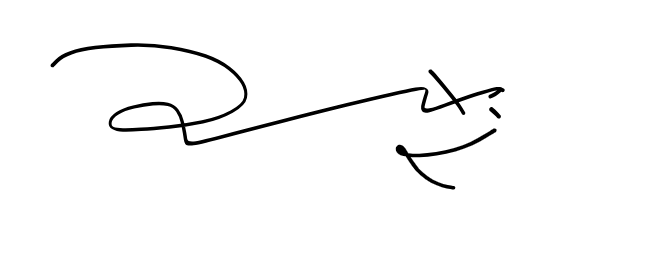
\includegraphics[width=6cm]{image/tandatangan.png}
\vspace{-1cm}

\underline{Ricky Wijaya} \\
NIM: 18222043